\chapter{Chapter Four Title}

\section{Typesetting Algorithms}

We can use the \emph{algorithm2e} package to typeset algorithm blocks in a way
that is pleasant to read. In listing \ref{alg:linear-search} we have an example
of a linear search algorithm typeset with \emph{algorithm2e}

\begin{function}[H]
  \For{$i \gets 0$ \KwTo $N$}{
    \If{$A[i] = e$} {
      \Return{true}
    }
  }
  \Return{false}
  \caption{LinearSearch($A,N,e$)}
  \label{alg:linear-search}
\end{function}

\section{Pictures are possible with TiKZ}

Any \LaTeX wouldn't be complete without an image drawn with TiKZ. Figure
\ref{fig:linear-search} shows the linear behavior of the Linear Search
algorithm.

\begin{figure}[h]
  \centering
  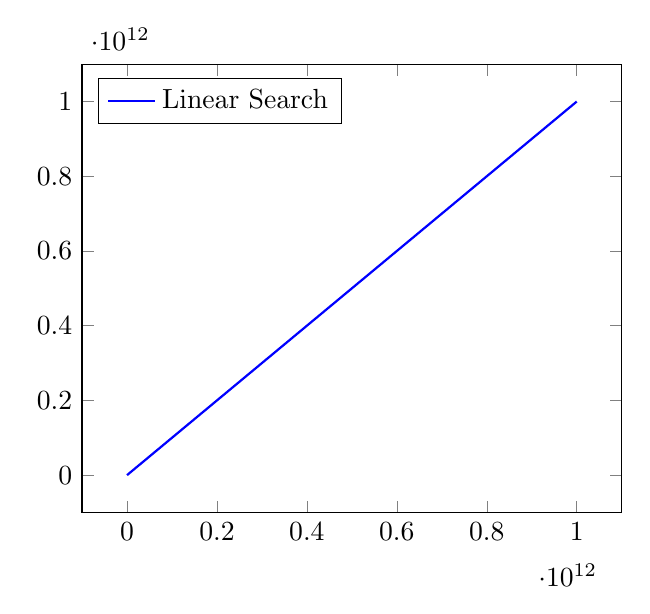
\begin{tikzpicture}
    \begin{axis}[
        legend pos=north west,
        legend cell align=left]
      \addplot[blue, thick, domain=1:1e12] {
        x
      };
      \addlegendentry{Linear Search};
    \end{axis}
  \end{tikzpicture}
  \caption{Linear Search Time Complexity}
  \label{fig:linear-search}
\end{figure}

